\chapter{Aspectos Conceituais}
Alguns dos principais conceitos para compreensão e contextualização deste projeto são trabalhados neste capítulo.

\section{Macacos e Reservas Naturais}
Para melhor compreensão do aspecto biológico que este trabalho toca, foi realizada uma entrevista com a professora Cristiane Pizzutto, que pode ser vista na íntegra no apêndice A deste documento.

A partir desta, foi possível quantificar alguns parâmetros importantes para o dimensionamento do projeto, tal como a quantidade comumente observada de animais em bandos de reservas e cativeiros, para qual foi assegurado que, considerando um bando de dez macacos, estaríamos abrangendo seguramente o suficiente.

Também foi possível notar como a tarefa de observação para aquisição de dados relativos aos animais, tais como sinais vitais, movimentação e alimentação, é exaustiva, toma tempo e pode ser objetiva o bastante para que possa ser realizada por um sistema remoto.

A parte subjetiva do levantamento de dados está relacionada às atividades e interações dos animais, que normalmente só podem ser adquiridos por observação direta. Essa é a parte que nosso projeto tenta abordar e que nos fez perceber que talvez, para cativeiro, o auxílio de câmeras com alguma inteligência seria bem vindo.

\section{Tecnologias Potenciais}
\textbf{Redes de Sensores Sem Fio}

A emergência da tecnologia de Redes de Sensores Sem Fio (RSSF) permitiu não somente o monitoramento das variáveis de um objeto, mas também o supervisionamento de todo o contexto em que ele está incluído e da interação dele com os demais pontos do sistema sendo sensoriados.

RSSFs são especialmente relevantes quando se tratando de ambientes cuja área que deve ser coberta é muito extensa. Estas redes são compostas por nós interligados, em que cada nó deve ter sensores, processamento, memória, antena e bateria independentes e sustentáveis.

Dada essa composição, as RSSFs são capazes de satisfazer áreas de cobertura muito extensas e são ótimas para criar integração entre elementos que estão, localmente, constantemente conjuntos.

Por isso, compõem uma tecnologia ótima para organizações biológicas, que envolvem grandes populações distribuídas, sendo, portanto, frequentemente aplicadas em sistemas agrícolas.

Como enfatizado por Handcock (2009) \cite{handcock}, para animais essa utilidade também é incluída, mas prevê algumas ressalvas. Uma delas considera a situação de que o animal de vida livre pode permanecer por semanas fora do alcance de pontos de acesso que recebam seus dados e, por esse motivo, cada nó da rede deverá possuir bateria e memória suficientemente robustas. Para reduzir o tempo de ausência de resposta de um determinado indivíduo, é possível implementar escuta nos próprios nós da rede, de forma que os animais que entrarem em contato entre si mantenham as informações dos demais, aumentando a chance de que algum deles possa transmiti-las para o servidor no alcance de pontos de acesso. Essa prática, no entanto, exige ainda mais energia e armazenamento.

RSSFs são, por vezes, estudadas para posicionamento em ambientes internos, principalmente atreladas ao uso de pontos de acesso \emph{Wi-fi}, que já são naturalmente alocados nesses espaços para uso de internet.

\textbf{Rádio}
A aplicação tecnológica para rastreamento de animais mostra-se insistente no uso de transmissores de rádio por muitos anos, por mais que a tecnologia de localização para aplicações humanas já o tenha superado de longe.

O RFID (\emph{Radio Frequency Identification}) foi bastante usado para obter informações relacionadas à condição do animal identificado. Recentemente, estes transmissores têm sido também utilizados para detectar encontros sociais entre animais através de picos de intensidade do sinal de rádio sendo transmitido.

\textbf{GPS}
A emancipação do GPS aplicado ao smartphone praticamente trivializou a tarefa de localização, principalmente quando associada à mobilidade e roteamento.

A integração de tal tecnologia em sistemas biológicos demonstra uma tentativa de integrar o sensoriamento da interação do animal com o ambiente, como é salientado por Handcock \cite{handcock}.

O GPS, no entanto, tem uma série de complicações. Primeiramente, sua precisão em baixa escala é bem complicada. Handcock afirma que para obter boa acurácia, é necessário ter uma taxa de amostragem relativamente alta, o que é bastante ruim para a sustentabilidade da memória e da energia do sistema.

Um outro problema está relacionado à pouca praticidade do módulo GPS, que apresenta peso relativamente elevado (aproximadamente 10g) dependendo do animal que está sendo rastreado.

\section{Modelos Comerciais}
Alguns modelos de coleiras voltadas a mamíferos são citadas na tabela 1. Os produtos são fornecidos pela empresa ATS (\emph{Animal Traceability Solutions}) \cite{ats} que, infelizmente, não discrimina o porte recomendado do animal usuário em seu site, portanto só foi possível inferir o peso que o dispositivo deste projeto deveria ter confirmando o que havia sido relatado pelos pesquisadores: de algo de no máximo 10g, uma vez que macacos menores pesam cerca de 400g.

Por outro lado, foi possível conceber alguns potenciais modelos para o invólucro do produto final deste projeto, principalmente no que diz respeito ao material utilizado.

\begin{table}[ht]
\centering
\caption{Exemplos comerciais de coleiras de rastreamento de mamíferos da ATS}
\vspace{0.5cm}
\begin{tabular}{l|ccc}
\hline
Nome & \makecell{SM17X0 Mammal \\ Collar, X-Small} & \makecell{M15X5 Mammal \\ Zip-Tie Collar} & \makecell{W500 Wildlink GPS \\ Logger, Small Collar} \\

Imagem & \makecell{\includegraphics[scale=0.5]{ATS1}} & \makecell{\includegraphics[scale=0.5]{ATS2}} & \makecell{\includegraphics[scale=0.5]{ATS3}}\\% \vspace{0.4cm}\\

Peso & 9 a 16g & 10 a 40g & 65 a 115g\\ %\vspace{0.4cm}\\

Bateria & Lítio / 156 a 282 dias & Lítio / 195 a 596 dias & AA / 1,75 a 3,5 anos \\%\vspace{0.4cm} \\

Material &
\makecell{- Coleira de \\ \textbf{neoprene} \\
- Encapsulamento \\ de resina a prova \\ de água} &
\makecell{ - Coleira de \textbf{tubo} \\ \textbf{de plástico (cable-tie)} \\
- Encapsulamento \\ de resina a prova \\ de água} &
\makecell{- Coleira de \textbf{neoprene} \\ \textbf{ou nylon} }
\end{tabular}
\vspace{0.4cm}\\
\centerline{\small{Fonte: autores}}
\end{table}

Como visto no item anterior, comercialmente é utilizado rádio na maior parte dos casos (M17X0 e M15X5) e, eventualmente, GPS (W500 - para o qual é possível notar que exige um peso bem superior ao limite estabelecido de cerca de 10g).
\FloatBarrier

\section{Algoritmos}
Inicialmente, é necessário compreender uma forma de calcular a posição dos animais através da distância entre macaco e ponto de acesso. De praxe, em RSSFs este cálculo pode ser feito de duas formas.

A primeira delas é utilizando a intensidade do sinal (\emph{Received Signal Strength Indication} - RSSI). O cálculo da distância, neste caso, é dado pelo seguinte modelo proposto pela \emph{Texas Instruments} (TI), que é melhor detalhado por Dong e Dargie (2012) \cite{dong}.

\begin{equation}
RSSI = -10 \times n \times \log_{10} d + A
\end{equation}

Sendo:
\begin{itemize}
\item d a distância em metros
\item RSSI a intensidade do sinal em dBm
\item n a constante de propagação do sinal
\item A a intensidade do sinal para 1 metro de distância
\end{itemize}

Essa é uma maneira simples de baixo custo de implementação, porém, como é bem destacado por Larsson (2015) \cite{larsson}, dada a alta variação de n devido a suscetibilidade do sinal à interferência do meio, demonstra-se um tanto imprecisa.

A constante de propagação pode ser determinada empiricamente. Se sabe n=2 para o vácuo; no ar, valores coerentes estão entre 2.7 e 4. A determinação da constante para este projeto pode ser observada no apêndice.

Outra forma seria calcular a distância sabendo a velocidade de propagação do sinal no meio, dado o tempo que demora para que o sinal seja recebido a partir da implementação de um eco. Idealmente esta é uma abordagem muito mais precisa, que só é impossibilitada em casos que o hardware utilizado não possua relógio. No entanto, qualquer deficiência na temporização e sincronização, por menor que seja, pode comprometer a precisão de tal metodologia.

Para este projeto, pretende-se implementar a primeira forma e verificar a precisão da mesma.

Além disso, foi requerido desenvolver um algoritmo para obtenção do mapeamento da posição dos macacos. Este tema já havia sido discutido por Amaral e Biscaro \cite{larissaamaralmiltonbiscaro} e, para este caso, o único algoritmo que se fez praticável é a trilateração.

\begin{figure}[ht]
  \centering
    \caption{Algoritmo de trilateração}
    \includegraphics[scale=1]{trilateracao}
	\centerline{\small{Fonte: autores}}
\end{figure}
\FloatBarrier

Dada a figura acima, o ponto P pode ser calculado conhecendo-se os pontos fixos P1, P2, P3, as distâncias entre eles e as distâncias entre os mesmos e P (r1, r2 e r3, respectivamente). Assim, é criado um sistema compondo as três equações de circunferências, resultando no seguinte equacionamento.

Se x1 $\neq$ x2:

\quad $\alpha = \dfrac{x1 - x3}{x2 - x1}$

\quad $\beta = 2 \times [(y3 - y1) + \alpha(y2 - y1)]$

\quad Se $\beta \neq$ 0:

\quad \quad y = $\dfrac{(x3^2 - x1^2) + (y3^2 - y1^2) + (r1^2 - r3^2) + \alpha[(x2^2 - x1^2) + (y2^2 - y1^2) + (r1^2 - r2^2)]}{\beta}$

\quad \quad x = $\dfrac{2y(y1 - y2) + (x2^2 - x1^2) + (y2^2 - y1^2) + (r1^2 - r2^2)}{2(x2 - x1)}$

Senão, se x2 $\neq$ x3:

\quad $\alpha = \dfrac{x1 - x3}{x3 - x2}$

\quad $\beta = 2 \times [(y3 - y1) + \alpha(y2 - y3)]$

\quad Se $\beta \neq$ 0:

\quad \quad y = $\dfrac{(x3^2 - x1^2) + (y3^2 - y1^2) + (r1^2 - r3^2) + \alpha[(x3^2 - x2^2) + (y3^2 - y2^2) + (r2^2 - r3^2)]}{\beta}$

\quad \quad x = $\dfrac{2y(y2 - y3) + (x3^2 - x2^2) + (y3^2 - y2^2) + (r2^2 - r3^2)}{2(x3 - x2)}$

Se não couberem nenhum desses dois casos, sabemos que as circunferências não possuem ponto de intersecção.

Enfim, sabendo que o sistema deve considerar o erro $\epsilon$ de cada distância medida, foi elaborado um algoritmo semelhante ao \emph{cellbased} \cite{larissaamaralmiltonbiscaro} que leva em conta as circunferências para raio r + $\epsilon$, tal como na figura a seguir.

\begin{figure}[ht]
  \centering
  \caption{\emph{Cellbased} - área de intersecção}
    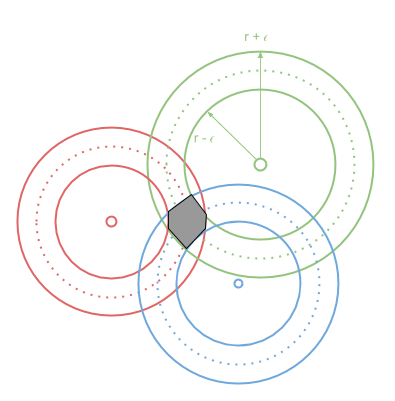
\includegraphics[scale=0.5]{cellbased}
	\centerline{\small{Fonte: autores}}
\end{figure}
\FloatBarrier

O ponto sensível dessa linha de pensamento é o fato que, devido às possíveis variâncias no erro, em alguns casos pode ocorrer o ilustrado abaixo, em que a área alvo não se fecha como deveria. Para estes casos é necessário tratamento especial, ou tentando inferir valores mais adequados por proximidade entre os pontos de intersecção par-a-par das circunferências ou simplesmente tomando-os como dados inválidos demais e descartando-os.

\begin{figure}[ht]
  \centering
    \caption{\emph{Cellbased} - área de intersecção fora do alcance}
    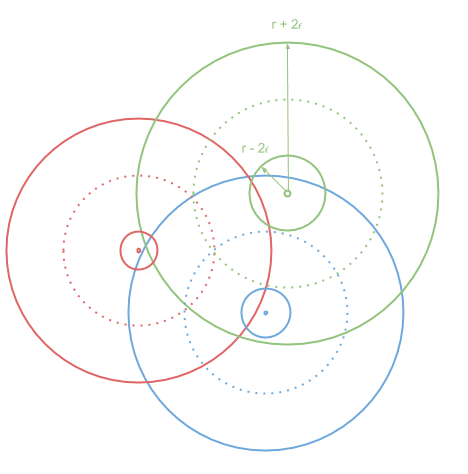
\includegraphics[scale=0.6]{cellbased-offrange}
	\centerline{\small{Fonte: autores}}
\end{figure}
\FloatBarrier
